\documentclass[%fontsize=12pt,
paper=a4,%Papierformat
parskip=half,%Abstand statt Einzug für Absatzwechsel
headsepline,%Linie unter Kopfzeile
plainheadsepline,%Linie unter Kopfzeile bei Kapitelanfängen
twoside=false,%Einseitiger Satz
headings=small%Kleine Kapitelüberschriften
]{scrreprt}

%%%PAKETE	
%%Grundlegende Pakete
\usepackage[utf8]{inputenc}%Eingabezeichensatz
\usepackage[T1]{fontenc}%Verwende Type 1-Schriften
\usepackage{lmodern}%Schriftart
\usepackage[ngerman]{babel}%Deutsche Silbentrennung
\usepackage{microtype}

%% Keine Warnings bei float
\usepackage{scrhack}

%%Pakete für Zeichen
\usepackage{textcomp}%Symbole
\usepackage{latexsym}%Symbole
\usepackage[style=german]{csquotes}%Anführungszeichen mit \enquote{}

%%Pakete für Schriften
\usepackage{color}

%%Pakete für Formatierung
\usepackage{scrpage2}%Paket für KOMA-Script Kopf- und Fußzeilen
\usepackage{geometry}%Seitenränder anpassen

%%Pakete für Tabellen
\usepackage{multirow}

%%Pakete für Mathematik
\usepackage{amsmath}%Mathematikpakte der AMS
\usepackage{amsfonts}%Schriften der AMS
\usepackage{amssymb}%Symbole der AMS

%%Pakete für Grafiken
\usepackage{graphicx}

%%Pakete für Quelltext
\usepackage{listings}

%%Sonstige Pakete
\usepackage[iso]{datetime}
\usepackage{ifthen}
\usepackage{caption}
\usepackage{subcaption}

%%%BEFEHLE
%%Befehl für typographisch korrekten Abstand bei Abkürzungen wie "z. B." oder "d. h."
\newcommand{\abk}[2]{{#1}.\,{#2}.}

%%Sonstige Befehle und Variablen
\newboolean{draft}

%%%EINSTELLUNGEN
%%Grundlegende Einstellungen für das Dokument
\setboolean{draft}{true}

\title{Laborbericht}
\subtitle{Komplexe Informationstechnische Systeme - Grundlagen}
\author{Lennard Pfennig \and Simon Buttgereit \and Michael Pfeiffer}
\date{TODO DATUM}
\subject{Sommersemester 2016}
\publishers{Version alpha}%raped field

% Wenn Boolean draft gesetzt ist, setze Hinweis auf Titelseite
\ifthenelse{\boolean{draft}}{%if then
	\titlehead{\centering{\textcolor{red}{
		{\Huge Entwurf}\\
		Kompiliert: \today \ \currenttime
	}}}
}{}

%%Schriftart
\renewcommand{\familydefault}{\sfdefault}%Serifenlose Schrift

%%Seitenrandeinstellungen
\geometry{a4paper,left=25mm,right=25mm, top=30mm, bottom=30mm}

%%Anpassungen von Kapitelüberschriften
\renewcommand*{\chapterheadstartvskip}{\vspace{-5mm}}

%%Anpassen von Kopf- Fußzeilen
\pagestyle{scrheadings}
\automark{chapter}
\ohead[\headmark]{\headmark}
\chead{}
% Wenn Boolean draft gesetzt ist, setze Hinweis auf jeder Seite oben links
\ifthenelse{\boolean{draft}}{%if then
	\ihead[\textnormal{\textcolor{red}{Entwurf - Kompiliert: \today \ \currenttime}}]
	{\textnormal{\textcolor{red}{Entwurf - Kompiliert: \today \ \currenttime}}}
}
{%else
	\ihead{}
}

%%Einstellungen für Quelltext
\lstset{ %
language=c++,%Standardsprache
basicstyle=\footnotesize\ttfamily,
breaklines=true,
%showstringspaces=false,
flexiblecolumns=true,
numbers=right,
numberstyle={\tiny}
}

%%Einstellungen für die PDF-Erzeugung
%Hyperref muss als letztes aufgerufen werden!
\usepackage[pdfstartview = FitH,%Seiten auf volle Breite anzeigen
bookmarksopen=true,bookmarksnumbered=true,%Inhaltsverzeichnis im PDF links anzeigen
colorlinks,linkcolor=black,plainpages=false,hypertexnames=false,citecolor=black,filecolor=black,urlcolor=black,%Keine Hervorhebung von Links
pdfpagelabels,pdftitle={Laborbericht},
pdfauthor={Lennard Pfennig, Simon Buttgereit und Michael Pfeiffer},
pdfsubject={Komplexe Informationstechnische Systeme}]{hyperref}%PDF-Informationen

\pdfcompresslevel=0%PDF-Kompression (Bilder)

\begin{document}
\maketitle

\tableofcontents

\chapter{Einleitung}
Dieser Laborbericht dokumentiert das Praktikum \enquote{Kugelfallversuch} zur Vorlesung \enquote{Komplexe Informationstechnische Systeme -- Grundlagen} der Gruppe im Sommersemester 2016.
Der Bericht umfasst (neben dieser Einleitung) drei Kapitel.

\cref{k_analyse} umfasst eine knappe Beschreibung des Versuchsaufbaus, TODO

Im darauffolgenden \cref{k_design} wird das entworfene Softwaresystem in seinem Aufbau und seiner Funktion beschrieben.
Anschließend werden die Grenzwerte, unter denen das System seine Funktion erfüllt, dargestellt und eine Fehlerbetrachtung durchgeführt.

In \cref{k_implementierung} wird schließlich die Implementierung des Systems detailliert und eine Validierung durchgeführt.

\chapter{Implementierung}



\begin{figure}[hb] \centering
	\begin{subfigure}[b]{0.4\textwidth}
  		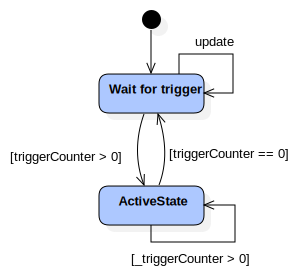
\includegraphics[width=\textwidth]{UML/fallcontroller_simple_loop_statechart.pdf}
		\caption{Einfache Darstellung}
		\label{uml:statechart_simleloop}
	\end{subfigure}\hspace{1cm}
	\begin{subfigure}[b]{0.4\textwidth}
 		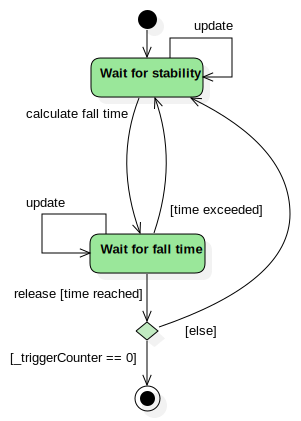
\includegraphics[width=\textwidth]{UML/fallcontroller_active_state_statechart.pdf}
  		\caption{Genauere Beschreibung des ActiveStates aus \ref{uml:statechart_simleloop}}
  		\label{uml:statechart_activeState}
	\end{subfigure}
	\caption{Beschreibung der Hauptschleife als State-Chart-Diagramm}
	\label{uml:statechart}
\end{figure}

\begin{figure}[hb] \centering
\end{figure}

\begin{figure}[hb] \centering
  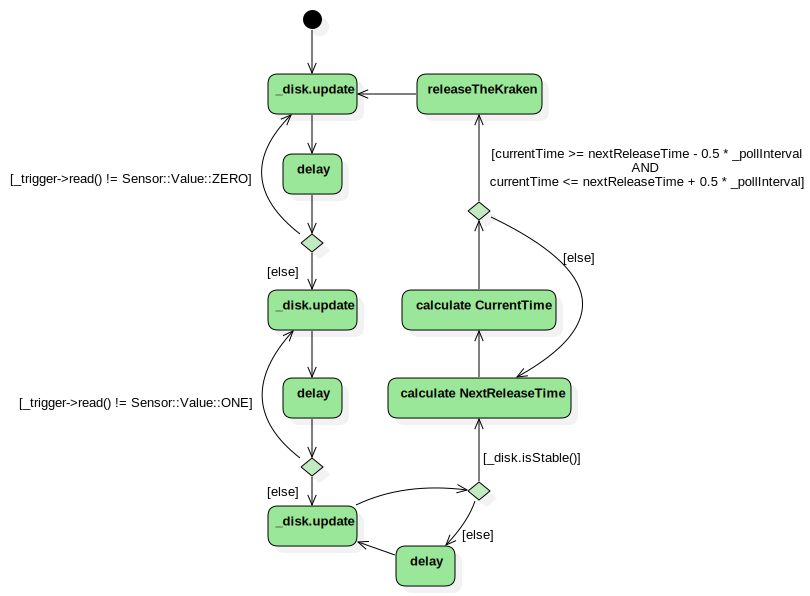
\includegraphics[width=\textwidth]{UML/fallcontroller_loop_activity_diagram.pdf}
  \caption{Genauere Beschreibung der Hauptschleife als Aktivitätsdiagramm}
  \label{uml:activity_diagram}
\end{figure}

\begin{figure}[hb] \centering
  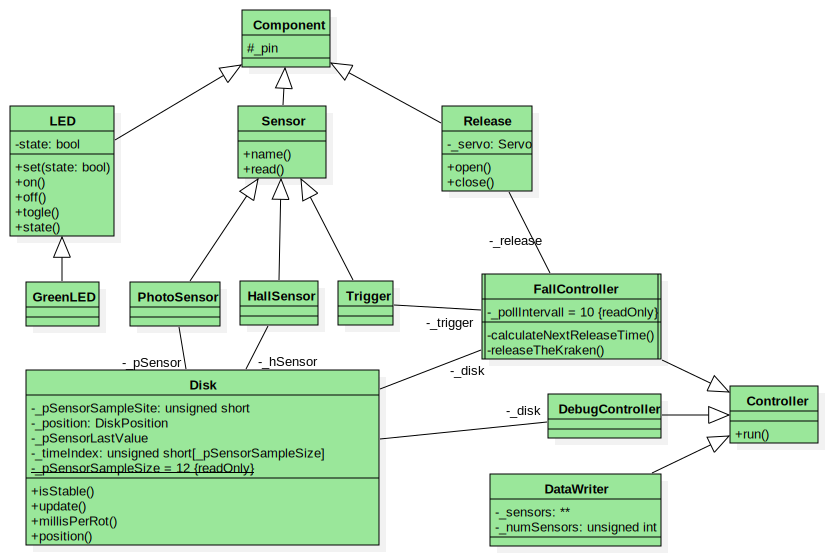
\includegraphics[width=\textwidth]{UML/class_diagram.pdf}
  \caption{Klassendiagramm der Implementierung}
  \label{uml:class_diagram}
\end{figure}


\end{document}
